\documentclass[11pt,a4paper]{article}
\usepackage[utf8]{inputenc}
\usepackage[vietnamese]{babel}
\usepackage{amsmath,amssymb}
\usepackage[version=4]{mhchem}
\usepackage{geometry}
\geometry{top=1.5cm,bottom=1.2cm,left=1.4cm,right=1.4cm,headheight=28pt,headsep=12pt,footskip=18pt}
\usepackage{graphicx}
\usepackage{xcolor}
\usepackage{tabularx}
\usepackage{array}
\usepackage{tikz}
\usepackage{fancyhdr}
\usepackage{enumitem}
\usepackage{multido}
\usepackage{tcolorbox}
\usepackage{colortbl}

\definecolor{hfRed}{HTML}{D32F2F}
\definecolor{hfGreen}{HTML}{8BC390}
\definecolor{mainGreen}{HTML}{2E7D32}
\definecolor{solBlue}{HTML}{1565C0}
\definecolor{tableGreen}{HTML}{E8F5E9}

\usepackage{ex_test}

\pagestyle{fancy}
\fancyhf{}
\renewcommand{\headrulewidth}{0.75pt}
\renewcommand{\headrule}{\hbox to\headwidth{\color{hfGreen}\leaders\hrule height \headrulewidth\hfill}}
\renewcommand{\footrulewidth}{0.75pt}
\renewcommand{\footrule}{\hbox to\headwidth{\color{hfGreen}\leaders\hrule height \footrulewidth\hfill}}

\fancyhead[L]{\small\itshape\color{hfRed}Tài liệu lưu hành nội bộ}
\fancyhead[R]{\small\color{hfRed}Thầy \textbf{TRẦN VĂN THẠNH} - 0777.470.803}

\fancyfoot[L]{\footnotesize\itshape\color{hfRed}CS1: 6/15 Nguyễn Hoàng, P. Kim Long, TP Huế \quad|\quad CS2: 24 Đặng Thái Thân, TP Huế}
\fancyfoot[R]{\small\textbf{\color{hfRed}Trang \thepage}}

\setlength{\parindent}{0pt}
\setlength{\parskip}{2pt}

\begin{document}

\begin{minipage}[t]{0.48\textwidth}
\textbf{TRƯỜNG THPT NGUYỄN HUỆ}\\
\textbf{TỔ LÍ -- HÓA -- CÔNG NGHỆ}\\
\textit{ĐỀ CHÍNH THỨC}\\
\textit{(Đề thi có 04 trang)}
\end{minipage}
\hfill
\begin{minipage}[t]{0.48\textwidth}
\raggedleft
\textbf{\color{hfRed}KIỂM TRA GIỮA KỲ I - NĂM HỌC 2026 - 2027}\\
\textbf{Môn: HÓA HỌC, Lớp 10}\\
\textit{Thời gian: 45 phút (không kể thời gian phát đề)}\\
\textbf{MÃ ĐỀ THI: 1203}
\end{minipage}

\vspace{4pt}
\noindent
\textit{Họ và tên thí sinh:} \dotfill \textit{SBD:} \dotfill

\vspace{2pt}
\noindent
\textit{\footnotesize (Cho biết nguyên tử khối: $\ce{H=1; B=10,81; C=12; N=14; O=16; F=19; Ne=20,19; Na=23; Mg=24; P=31; S=32; Cl=35,5; K=39; Ca=40; Br=79,91}$).}

\vspace{2pt}
\begin{center}
\textbf{CHÚ Ý: Học sinh không được sử dụng bảng tuần hoàn các nguyên tố hóa học.}
\end{center}

\vspace{2pt}
\hrule color{hfGreen} height 0.5pt

\vspace{4pt}
\begin{center}
\textbf{\color{hfRed}\large (BẢN GIÁO VIÊN -- CÓ LỜI GIẢI CHI TIẾT)}
\end{center}

\vspace{2pt}
\begin{center}
{\color{hfRed}\textbf{\large BẢNG ĐÁP ÁN RÚT GỌN (DÀNH CHO GIÁO VIÊN)}}
\end{center}

\vspace{2pt}
\noindent
\textbf{\color{mainGreen}1. Phần I: Trắc nghiệm nhiều lựa chọn (3,0 điểm - mỗi câu đúng 0,25 điểm)}
\begin{center}
\renewcommand{\arraystretch}{1.2}
\begin{tabular}{|c|c|c|c|c|c|c|c|c|c|c|c|c|}
\hline
\rowcolor{tableGreen}
\textbf{Câu} & \textbf{1} & \textbf{2} & \textbf{3} & \textbf{4} & \textbf{5} & \textbf{6} & \textbf{7} & \textbf{8} & \textbf{9} & \textbf{10} & \textbf{11} & \textbf{12} \\
\hline
\textbf{Đ/A} & \textbf{\color{hfRed}B} & \textbf{\color{hfRed}A} & \textbf{\color{hfRed}D} & \textbf{\color{hfRed}A} & \textbf{\color{hfRed}B} & \textbf{\color{hfRed}B} & \textbf{\color{hfRed}D} & \textbf{\color{hfRed}A} & \textbf{\color{hfRed}B} & \textbf{\color{hfRed}D} & \textbf{\color{hfRed}B} & \textbf{\color{hfRed}C} \\
\hline
\end{tabular}
\end{center}

\vspace{2pt}
\noindent
\textbf{\color{mainGreen}2. Phần II: Trắc nghiệm Đúng / Sai (2,0 điểm)}
\begin{center}
\renewcommand{\arraystretch}{1.2}
\begin{tabular}{|c|c|c|c|c|}
\hline
\rowcolor{tableGreen}
\textbf{Câu} & \textbf{Lệnh a)} & \textbf{Lệnh b)} & \textbf{Lệnh c)} & \textbf{Lệnh d)} \\
\hline
\textbf{Câu 1} & \textbf{\color{solBlue}SAI} & \textbf{\color{hfRed}ĐÚNG} & \textbf{\color{solBlue}SAI} & \textbf{\color{hfRed}ĐÚNG} \\
\hline
\textbf{Câu 2} & \textbf{\color{hfRed}ĐÚNG} & \textbf{\color{solBlue}SAI} & \textbf{\color{solBlue}SAI} & \textbf{\color{solBlue}SAI} \\
\hline
\end{tabular}
\end{center}

\vspace{2pt}
\noindent
\textbf{\color{mainGreen}3. Phần III: Trả lời ngắn (2,0 điểm - mỗi câu đúng 0,5 điểm)}
\begin{center}
\renewcommand{\arraystretch}{1.2}
\begin{tabular}{|c|c|c|c|c|}
\hline
\rowcolor{tableGreen}
\textbf{Câu} & \textbf{Câu 1} & \textbf{Câu 2} & \textbf{Câu 3} & \textbf{Câu 4} \\
\hline
\textbf{Đáp án} & \textbf{\color{hfRed}4} & \textbf{\color{hfRed}58} & \textbf{\color{hfRed}1} & \textbf{\color{hfRed}2} \\
\hline
\end{tabular}
\end{center}

\vspace{4pt}
\hrule color{hfGreen} height 0.5pt

\vspace{4pt}
\noindent
{\color{mainGreen}\textbf{\Large A. PHẦN TRẮC NGHIỆM (7 ĐIỂM)}}

\vspace{3pt}
\noindent
{\color{mainGreen}\textbf{\large PHẦN I. Câu trắc nghiệm nhiều phương án lựa chọn (3,0 điểm)}}\\
\textit{\small Thí sinh trả lời từ câu 1 đến câu 12. Mỗi câu hỏi thí sinh chỉ chọn một phương án.}
\vspace{2pt}

\begin{ex}
Phát biểu nào sau đây không đúng?
\choice
{Hạt proton và hạt neutron có khối lượng gần bằng nhau.}
{\True Khối lượng nguyên tử tập trung chủ yếu ở lớp vỏ.}
{Khối lượng hạt electron nhỏ hơn nhiều so với khối lượng hạt proton.}
{Trong nguyên tử, khối lượng tập trung chủ yếu ở hạt nhân.}

\loigiai{
Khối lượng nguyên tử tập trung chủ yếu ở hạt nhân vì khối lượng electron ở vỏ rất bé ($m_e \approx 0,00055\text{ amu}$). Phát biểu B sai.\\
\textbf{Chọn B.}
}
\end{ex}
\begin{ex}
Cho các phát biểu về sự chuyển động của electron trong nguyên tử như sau:\\
(a) Theo mô hình hành tinh nguyên tử, các electron chuyển động xung quanh hạt nhân theo những quỹ đạo tròn hay bầu dục.\\
(b) Theo mô hình hiện đại, các electron chuyển động rất nhanh xung quanh hạt nhân theo một quỹ đạo xác định tạo thành đám mây electron.\\
(c) Theo mô hình hiện đại, trong nguyên tử, electron chuyển động rất nhanh, không theo quỹ đạo xác định.\\
(d) Theo mô hình hiện đại, xác suất tìm thấy electron tại mỗi điểm trong không gian của AO là 90\%.\\
Số phát biểu đúng là
\choice
{\True 2.}
{3.}
{1.}
{4.}

\loigiai{
- (a) Đúng: Mô hình hành tinh nguyên tử (Rutherford -- Bohr) quy định quỹ đạo tròn hoặc elip.\\
- (b) Sai: Theo mô hình hiện đại, electron chuyển động không theo quỹ đạo xác định.\\
- (c) Đúng: Electron chuyển động rất nhanh và không theo quỹ đạo xác định.\\
- (d) Sai: Vùng không gian AO có xác suất tìm thấy khoảng 90\%, không phải tại mỗi điểm.\\
Có 2 phát biểu đúng là (a) và (c).\\
\textbf{Chọn A.}
}
\end{ex}
\begin{ex}
Hạt mang điện trong hạt nhân nguyên tử là
\choice
{neutron.}
{neutron và electron.}
{electron.}
{\True proton.}

\loigiai{
Hạt nhân nguyên tử chỉ chứa proton mang điện dương và neutron không mang điện. Do đó hạt mang điện trong hạt nhân chỉ có proton.\\
\textbf{Chọn D.}
}
\end{ex}
\begin{ex}
Trong bảng tuần hoàn các nguyên tố hóa học do nhà hóa học người Nga D. I. Mendeleev (1834 -- 1907) đề xuất năm 1869, các nguyên tố được sắp xếp theo chiều tăng dần của
\choice
{\True khối lượng nguyên tử.}
{số electron hóa trị.}
{số hiệu nguyên tử.}
{bán kính nguyên tử.}

\loigiai{
Bảng tuần hoàn của Mendeleev năm 1869 sắp xếp theo chiều tăng dần của khối lượng nguyên tử.\\
\textbf{Chọn A.}
}
\end{ex}
\begin{ex}
Trong nguyên tử, vùng không gian bao quanh hạt nhân và mang điện tích âm được tạo nên bởi các hạt
\choice
{neutron.}
{\True electron.}
{alpha.}
{proton.}

\loigiai{
Vỏ nguyên tử bao quanh hạt nhân mang điện tích âm, tạo nên bởi các hạt electron.\\
\textbf{Chọn B.}
}
\end{ex}
\begin{ex}
Đường kính của nguyên tử khoảng $10^2\text{ pm}$, trong khi đường kính của hạt nhân khoảng $10^{-2}\text{ pm}$. Đường kính nguyên tử lớn gấp bao nhiêu lần so với đường kính hạt nhân?
\choice
{10.}
{\True 10000.}
{1000.}
{100.}

\loigiai{
$d_{\text{nguyên tử}} / d_{\text{hạt nhân}} = 10^2 / 10^{-2} = 10^4 = 10\,000\text{ (lần)}$.\\
\textbf{Chọn B.}
}
\end{ex}
\begin{ex}
Số electron tối đa có trong 1 AO p là
\choice
{3.}
{6.}
{1.}
{\True 2.}

\loigiai{
Theo nguyên lí Pauli, mỗi 1 orbital nguyên tử (AO) chỉ chứa tối đa 2 electron.\\
\textbf{Chọn D.}
}
\end{ex}
\begin{ex}
Bảng tuần hoàn các nguyên tố hóa học hiện nay gồm có
\choice
{\True 7 chu kì và 18 cột.}
{8 chu kì và 18 nhóm.}
{7 chu kì và 8 nhóm.}
{6 chu kì và 16 nhóm.}

\loigiai{
Bảng tuần hoàn hiện nay gồm có 7 chu kì và 18 cột.\\
\textbf{Chọn A.}
}
\end{ex}
\begin{ex}
Phát biểu nào sau đây không đúng khi nói về vai trò của hóa học đối với đời sống và sản xuất?
\choice
{Nghiên cứu và sản xuất các loại thuốc chữa bệnh, vắc-xin và vật tư y tế.}
{\True Nghiên cứu quy luật hình thành, vận động của các thiên thể và địa tầng Trái Đất.}
{Tạo ra các sản phẩm tiêu dùng thiết yếu như xà phòng, chất tẩy rửa và chất dẻo.}
{Cung cấp phân bón hóa học và thuốc bảo vệ thực vật nhằm tăng năng suất nông nghiệp.}

\loigiai{
Nghiên cứu thiên thể thuộc Thiên văn học; nghiên cứu địa tầng thuộc Địa chất học.\\
\textbf{Chọn B.}
}
\end{ex}
\begin{ex}
Kí hiệu phân lớp electron nào sau đây không đúng?
\choice
{3d.}
{3s.}
{3p.}
{\True 3f.}

\loigiai{
Lớp thứ 3 ($n = 3$) chỉ gồm các phân lớp 3s, 3p, 3d; không có phân lớp 3f.\\
\textbf{Chọn D.}
}
\end{ex}
\begin{ex}
Cho các nguyên tử: $^{12}_6\ce{X}, ^{14}_7\ce{Y}, ^{14}_6\ce{Z}, ^{24}_{12}\ce{T}$. Các nguyên tử thuộc cùng một nguyên tố hóa học là
\choice
{\ce{Y} và \ce{Z}.}
{\True \ce{X} và \ce{Z}.}
{\ce{Z} và \ce{T}.}
{\ce{X} và \ce{T}.}

\loigiai{
$^{12}_6\ce{X}$ và $^{14}_6\ce{Z}$ đều có số proton $Z = 6$ (nguyên tố Carbon - $\ce{C}$) nên thuộc cùng một nguyên tố hóa học.\\
\textbf{Chọn B.}
}
\end{ex}
\begin{ex}
X là nguyên tố s. Trong bảng tuần hoàn, X có thể thuộc nhóm
\choice
{IB.}
{VIB.}
{\True IA.}
{VIA.}

\loigiai{
Nguyên tố s thuộc phân nhóm chính nhóm IA hoặc IIA (và He ở nhóm VIIIA). Do đó X có thể thuộc nhóm IA.\\
\textbf{Chọn C.}
}
\end{ex}
\vspace{4pt}
\noindent
{\color{mainGreen}\textbf{\large PHẦN II. Câu trắc nghiệm đúng sai (2,0 điểm)}}\\
\textit{\small Thí sinh trả lời từ câu 1 đến câu 2. Trong mỗi ý a), b), c), d) ở mỗi câu, thí sinh chọn đúng hoặc sai.}
\vspace{2pt}

\begin{ex}
Fluorine và hợp chất của nó được sử dụng làm chất chống sâu răng, chất cách điện, chất làm lạnh, vật liệu chống dính, \dots\ Nguyên tử fluorine (\ce{F}) chứa 9 electron và có số khối là 19.
\choiceTF
{Nguyên tử \ce{F} có điện tích lớp vỏ là +9}
{\True Hạt nhân nguyên tử \ce{F} có 9 proton và 10 neutron}
{Khối lượng của một nguyên tử \ce{F} xấp xỉ 28 amu}
{\True Phân tử $\ce{RF2}$ có tổng số hạt mang điện là 60. Nguyên tử của nguyên tố R có 2 electron thuộc lớp M và R là nguyên tố kim loại}

\loigiai{
a) \textbf{SAI}: Điện tích lớp vỏ là $-9$ (hoặc $-9e$), không phải $+9$.\\
b) \textbf{ĐÚNG}: $Z = 9 \implies p = 9$; neutron $N = 19 - 9 = 10$.\\
c) \textbf{SAI}: Khối lượng xấp xỉ số khối $A = 19\text{ amu}$.\\
d) \textbf{ĐÚNG}: Trong $\ce{RF2}$, tổng hạt mang điện: $2Z_R + 36 = 60 \implies Z_R = 12$ (Mg: $\ce{1s^2 2s^2 2p^6 3s^2}$). Lớp M có 2 electron, là kim loại.
}
\end{ex}
\begin{ex}
Boron (\ce{B}) là nguyên tố có nhiều tác dụng đối với cơ thể người như: làm lành vết thương, điều hoà nội tiết sinh dục, chống viêm khớp, \dots\ Do ngọn lửa cháy có màu đặc biệt nên boron vô định hình được dùng làm pháo hoa. Boron có hai đồng vị là $^{10}_5\ce{B}$ và $^{11}_5\ce{B}$, nguyên tử khối trung bình là 10,81.
\choiceTF
{\True Hai đồng vị của boron có cùng số proton nhưng khác nhau về số neutron}
{Nguyên tử của nguyên tố \ce{B} có 4 electron s và có 3 electron ở phân lớp ngoài cùng}
{Nguyên tố \ce{B} thuộc chu kì 3 trong bảng tuần hoàn}
{Phần trăm số nguyên tử của đồng vị $^{10}_5\ce{B}$ trong tự nhiên là 81\%}

\loigiai{
a) \textbf{ĐÚNG}: Cùng số proton ($Z = 5$), khác số neutron ($N = 5$ và $N = 6$).\\
b) \textbf{SAI}: Cấu hình B: $\ce{1s^2 2s^2 2p^1}$, phân lớp ngoài cùng là $2p$ chỉ có 1 electron.\\
c) \textbf{SAI}: Có 2 lớp electron nên thuộc chu kì 2.\\
d) \textbf{SAI}: Đồng vị $^{10}_5\ce{B}$ chiếm 19\%, $^{11}_5\ce{B}$ chiếm 81\%.
}
\end{ex}
\vspace{4pt}
\noindent
{\color{mainGreen}\textbf{\large PHẦN III. Câu trắc nghiệm yêu cầu trả lời ngắn (2,0 điểm)}}\\
\textit{\small Thí sinh trả lời từ câu 1 đến câu 4.}
\vspace{2pt}

\begin{ex}
Nguyên tử của nguyên tố calcium ($Z = 20$) có bao nhiêu lớp electron?

\loigiai{
Cấu hình electron Ca ($Z = 20$): $\ce{1s^2 2s^2 2p^6 3s^2 3p^6 4s^2} \implies$ có 4 lớp electron.\\
\textbf{Đáp án: 4.}
}
\end{ex}
\begin{ex}
Cho biết tổng số hạt proton, neutron và electron trong một nguyên tử của nguyên tố $^{39}_{19}\ce{K}$ là bao nhiêu?

\loigiai{
Trong nguyên tử $^{39}_{19}\ce{K}$: $p = e = 19$, $n = 39 - 19 = 20 \implies S = 19 + 19 + 20 = 58$.\\
\textbf{Đáp án: 58.}
}
\end{ex}
\begin{ex}
Trong tự nhiên, nguyên tố bromine có 2 đồng vị là $^{79}_{35}\ce{Br}$ và $^{81}_{35}\ce{Br}$. Nguyên tử khối trung bình của bromine là 79,91. Trong hợp chất $\ce{NaBrO}_x$, nguyên tử đồng vị $^{81}\ce{Br}$ chiếm 30,994\% về khối lượng. Giá trị của $x$ là bao nhiêu (với O và Na là các đồng vị $^{16}_8\ce{O}, ^{23}_{11}\ce{Na}$)?

\loigiai{
Tỉ lệ đồng vị $^{81}\ce{Br}$ là 45,5\%.\\
$$\%m_{^{81}\ce{Br}} = \frac{81 \times 0,455}{23 + 79,91 + 16x} \times 100\% = 30,994\% \implies 102,91 + 16x \approx 118,91 \implies x = 1.$$
\textbf{Đáp án: 1.}
}
\end{ex}
\begin{ex}
Cho các nguyên tử sau: $\ce{X}\ (Z = 11); \ce{Y}\ (Z = 17); \ce{Z}\ (Z = 20); \ce{T}\ (Z = 26)$. Có bao nhiêu nguyên tố thuộc loại nguyên tố s?

\loigiai{
$\ce{X}\ (Z = 11: \ce{[Ne]3s^1})$ và $\ce{Z}\ (Z = 20: \ce{[Ar]4s^2})$ là nguyên tố s.\\
Vậy có 2 nguyên tố thuộc loại nguyên tố s.\\
\textbf{Đáp án: 2.}
}
\end{ex}
\vspace{6pt}
\noindent
{\color{mainGreen}\textbf{\Large B. PHẦN TỰ LUẬN (3 ĐIỂM)}}
\vspace{3pt}

\begin{ex}
\textbf{(1,0 điểm)} Phosphorus (P) là một nguyên tố dinh dưỡng khoáng thiết yếu cho sự phát triển của cây trồng, thường có mặt trong các loại phân bón NPK. Trong bảng tuần hoàn, nguyên tố phosphorus có số hiệu nguyên tử là 15.\\
a) Viết cấu hình electron nguyên tử của P ở trạng thái cơ bản.\\
b) Xác định vị trí của P (chu kì và nhóm) trong bảng tuần hoàn, cho biết P thuộc loại nguyên tố nào (s, p hay d)?

\loigiai{
a) Cấu hình electron nguyên tử của P ($Z = 15$):\\
$\ce{1s^2 2s^2 2p^6 3s^2 3p^3}$ (hoặc $[\ce{Ne}]\ce{3s^2 3p^3}$). \hfill \textit{(0,5 điểm)}\\
b) Vị trí của P trong bảng tuần hoàn:\\
- Ô nguyên tố: số 15 (vì $Z = 15$).\\
- Chu kì: Chu kì 3 (vì có 3 lớp electron).\\
- Nhóm: Nhóm VA (vì có 5 electron hóa trị ở lớp ngoài cùng $\ce{3s^2 3p^3}$, electron cuối cùng điền vào phân lớp p).\\
- P là nguyên tố p. \hfill \textit{(0,5 điểm)}
}
\end{ex}
\begin{ex}
\textbf{(1,0 điểm)} Neon (Ne) là một nguyên tố khí hiếm, phát ra ánh sáng đỏ cam đặc trưng khi có phóng điện qua khí ở áp suất thấp và được ứng dụng trong một số loại biển hiệu phát sáng. Neon có ba đồng vị bền và tỉ lệ phần trăm số nguyên tử các đồng vị của Ne được xác định theo phổ khối lượng như hình sau:
\begin{center}
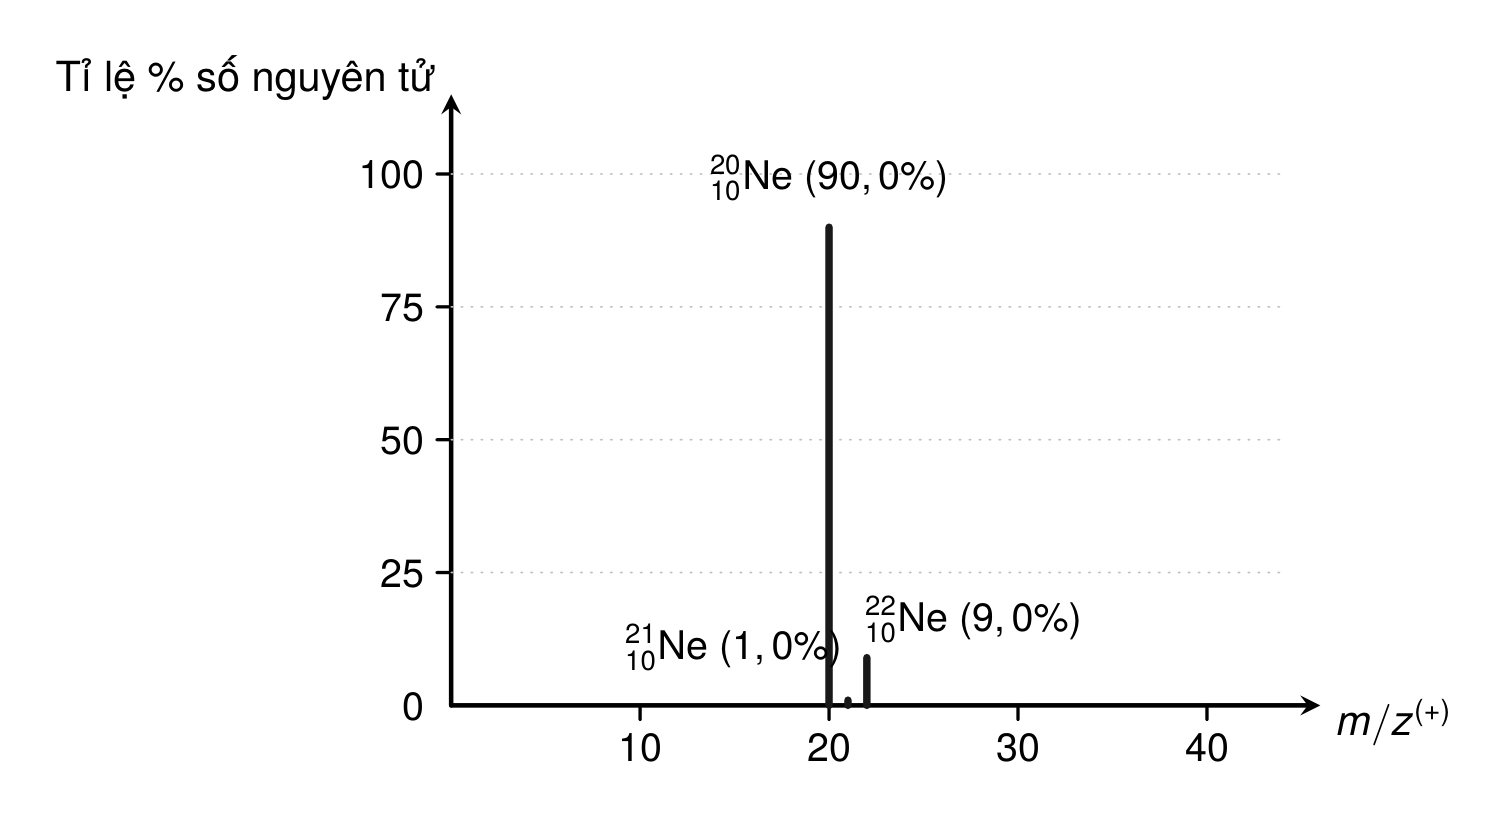
\includegraphics[width=8.5cm]{images_hoa10/pho_khoi_luong_neon_1201.png}
\end{center}
a) Tính nguyên tử khối trung bình của Neon (kết quả làm tròn đến hàng phần trăm).\\
b) Tính số nguyên tử của mỗi loại đồng vị còn lại khi có 1 nguyên tử $^{21}_{10}\ce{Ne}$ (kết quả làm tròn đến hàng đơn vị).\\
c) Tính thể tích của 10 gam Ne ở điều kiện chuẩn ($25^\circ\text{C}$, 1 bar) (kết quả làm tròn đến hàng phần mười).

\loigiai{
Dựa vào phổ khối lượng: $^{20}_{10}\ce{Ne}$ (90,0\%); $^{21}_{10}\ce{Ne}$ (1,0\%); $^{22}_{10}\ce{Ne}$ (9,0\%).\\
a) Nguyên tử khối trung bình của Neon:
$$\overline{A}_{\ce{Ne}} = \frac{20 \times 90,0 + 21 \times 1,0 + 22 \times 9,0}{100} = \frac{2019}{100} = 20,19. \hfill \textit{(0,4 điểm)}$$
b) Tỉ lệ số nguyên tử của 3 đồng vị là $90 : 1 : 9$.\\
Khi có 1 nguyên tử $^{21}_{10}\ce{Ne}$ thì có tương ứng:
- 90 nguyên tử $^{20}_{10}\ce{Ne}$.
- 9 nguyên tử $^{22}_{10}\ce{Ne}$. \hfill \textit{(0,3 điểm)}\\
c) Số mol của 10 gam Ne: $n = \frac{10}{20,19} \approx 0,4953\text{ mol.}$\\
Ở điều kiện chuẩn ($25^\circ\text{C}$, 1 bar):
$$V = 0,4953 \times 24,79 \approx 12,278 \approx 12,3\text{ (lít)}. \hfill \textit{(0,3 điểm)}$$
}
\end{ex}
\begin{ex}
\textbf{(1,0 điểm)} Nguyên tố R thuộc nhóm A trong bảng tuần hoàn. Nguyên tử R có tổng số electron ở các phân lớp s là 7 và tổng số electron ở lớp ngoài cùng là 1.\\
a) Viết cấu hình electron đầy đủ của nguyên tử R. Dự đoán tính chất hóa học cơ bản của nguyên tố R (kim loại hay phi kim) và giải thích.\\
b) Phân tử $\ce{R2XY4}$ có tổng số hạt proton là 86. Biết nguyên tố X và Y thuộc cùng một nhóm A và ở hai chu kì liên tiếp trong bảng tuần hoàn. Hãy xác định số hiệu nguyên tử của X và Y.

\loigiai{
a) Cấu hình electron đầy đủ của R: $\ce{1s^2 2s^2 2p^6 3s^2 3p^6 4s^1}$ (Potassium - K, $Z = 19$).\\
R là một kim loại kiềm mạnh, do bán kính nguyên tử lớn, năng lượng ion hóa nhỏ nên dễ nhường 1e tạo thành cation $\ce{K^+}$: $\ce{R \to R^+ + 1e}$. \hfill \textit{(0,5 điểm)}\\
b) Xác định số hiệu nguyên tử của X và Y:\\
Tổng số hạt proton: $2 \times 19 + Z_X + 4Z_Y = 86 \implies Z_X + 4Z_Y = 48$.\\
X và Y cùng nhóm A ở hai chu kì liên tiếp nhỏ: $|Z_X - Z_Y| = 8$.\\
Với $Z_X = Z_Y + 8 \implies (Z_Y + 8) + 4Z_Y = 48 \implies 5Z_Y = 40 \implies Z_Y = 8$ (Oxygen - O) và $Z_X = 16$ (Sulfur - S).\\
Kiểm tra: O ($Z=8$, chu kì 2, nhóm VIA) và S ($Z=16$, chu kì 3, nhóm VIA) thỏa mãn (hợp chất là $\ce{K2SO4}$).\\
Vậy: $Z_X = 16$ (Sulfur) và $Z_Y = 8$ (Oxygen). \hfill \textit{(0,5 điểm)}
}
\end{ex}
\vspace{6pt}
\begin{center}
\textbf{---------- HẾT ----------}\\
\textit{\small - Thí sinh không được sử dụng tài liệu.\\
- Giám thị không giải thích gì thêm.}
\end{center}
\end{document}
